\documentclass[a4paper, 12pt]{article}
\usepackage[T2A,T1]{fontenc}
\usepackage[utf8]{inputenc}
\usepackage[english, russian]{babel}
\usepackage{graphicx}
\usepackage[hcentering, bindingoffset = 10mm, right = 15 mm, left = 15 mm, top=20mm, bottom = 20 mm]{geometry}
\usepackage{multirow}
\usepackage{lipsum}
\usepackage{amsmath, amstext}
\usepackage{siunitx}
\usepackage{subcaption}
\usepackage{wrapfig}
\usepackage{adjustbox}
\usepackage{enumerate, indentfirst, float}
\usepackage{capt-of, svg}
\usepackage{icomma}

\newenvironment{bottompar}{\par\vspace*{\fill}}{\clearpage}
 
\begin{document}
\begin{titlepage}

\newcommand{\HRule}{\rule{\linewidth}{0.5mm}} % Defines a new command for the horizontal lines, change thickness here

\center % Center everything on the page
 
%----------------------------------------------------------------------------------------
%	HEADING SECTIONS
%----------------------------------------------------------------------------------------

\textsc{\LARGE Московский Физико-Технический Институт}\\[1,5cm] % Name of your university/college
\textsc{\Large Кафедра общей физики}\\[0.5cm] % Major heading such as course name
\textsc{\large Лабораторная работа \textnumero  3.3.4}\\[0.5cm] % Minor heading such as course title

%----------------------------------------------------------------------------------------
%	TITLE SECTION
%----------------------------------------------------------------------------------------

\HRule
\\[0.4cm]
{ \huge \bfseries Эффект Холла в полупроводниках}
\\[0.2cm] % Title of your document
\HRule
\\[1.5cm]


 
%----------------------------------------------------------------------------------------
%	AUTHOR SECTION
%----------------------------------------------------------------------------------------

\begin{minipage}{0.4\textwidth}
	\begin{flushleft} \large
		\emph{Автор:}\\
		Ришат \textsc{Исхаков} \\
		513 группа
	\end{flushleft}
\end{minipage}
~
\begin{minipage}{0.4\textwidth}
	\begin{flushright} \large
		\emph{Преподаватель:} \\
		Александр Александрович \textsc{Казимиров} % Supervisor's Name
	\end{flushright}
\end{minipage}

\begin{bottompar}
	\begin{center}
		
\includegraphics[width = 80 mm]{logo.jpg}
	\end{center}
	{\large \today}

\end{bottompar}
\vfill % Fill the rest of the page with whitespace

\end{titlepage}

\section{Цель работы}
Измерение подвижности и концентрации носителей заряда в полупроводниках.

В работе используются: \textit{электромагнит с источником питания, амперметр, миллиамперметр, милливеберметр, реостат, цифровой вольтметр, источник питания, образцы легированного германия.}


\subsection*{Теоретическая часть}

\subsubsection*{Дырки}

Эффект Холла, возникающий в проводниках, происходит из-за наличия некоторого количества свободных электронов в зоне проводимости и такого же количества дырок в валентной зоне. Чтобы понять причину образования дырок, нужно рассмотреть дырочную проводимость.


Дырочную проводимость можно объяснить при помощи следующей аналогии: если представить ряд людей, сидящих в аудитории, где нет запасных стульев. Когда кто-нибудь из середины ряда хочет уйти, он перелезает через спинку стула в пустой ряд и уходит. Здесь пустой ряд — аналог зоны проводимости, а ушедшего человека можно сравнить со свободным электроном.
Теперь представим, что ещё кто-то пришёл и хочет сесть. Из пустого ряда плохо видно, поэтому там он не садится. Вместо этого человек, сидящий возле свободного стула, пересаживается на него, вслед за ним это повторяют и все его соседи. Таким образом, пустое место как бы двигается к краю ряда. Когда это место окажется рядом с новым зрителем, он сможет сесть.
В этом процессе каждый сидящий передвинулся вдоль ряда. Если бы зрители обладали отрицательным зарядом, такое движение было бы  \textit{электрической проводимостью}. Если вдобавок стулья заряжены положительно, то ненулевым суммарным зарядом будет обладать только свободное место. Это простая модель, показывающая как работает \textit{дырочная проводимость}. Однако на самом деле, из-за свойств кристаллической решётки, дырка не локализована в определённом месте, как описано выше, а размазана по области размером во много сотен элементарных ячеек.


\begin{equation}
J \ddot{\varphi} + \dfrac{\left(BSN\right)^2}{R_{\Sigma}} \dot{\varphi} + D\varphi = BSNI
\end{equation}
$D$ - модуль кручения нити, $\varphi$ - угол поворота рамки от положения равновесия, $B$ - индукция магнитного поля, $N$ - число витков рамки, $I$ - ток в рамке, $S$ - площадь одного витка рамки, $R_{\Sigma}$ - полное сопротивление цепи, $J$ - момент инерции подвижной системы.
Введем обозначения:

\begin{equation}
\left.
\begin{aligned}
&\dfrac{(BSN)^2}{JR_{\Sigma}} = 2\gamma \\
&\dfrac{D}{J} = \omega_0^2 \\
&\dfrac{BSN}{J} = K 
\end{aligned}
\right\}
\end{equation}

Тогда уравнение движения рамки примет вид:
\begin{equation}
\label{eq:diff}
\ddot{\varphi} +2\gamma\dot{\varphi} + \omega_0^2 \varphi = KI
\end{equation}
Величина $\gamma$ называется \textit{коэффициентом затухания} подвижной системы гальванометра,  $\omega_0$ - собственной частотой колебаний рамки.

\subsubsection*{Режим измерения постоянного тока}
При измерении в режиме постоянного тока, когда затухают колебания: $\ddot{\varphi} = \dot{\varphi} = 0$, поэтому угол поворота можно определить формулой:
$$\varphi = \dfrac{KI}{\omega_0^2} = \dfrac{I}{C_I}$$

Постоянная $C_I = D/BSN$ называется динамической постоянной гальванометра.

\subsubsection*{Свободные колебания рамки}

В отсутствии внешних источников тока ($I = 0$) будем исследовать свободное движение рамки.
Если считать, что $\varphi(0) = 0$, $\dot{\varphi} = \dot{\varphi_0}$, уравнение примет вид:
$$\ddot{\varphi} +2 \gamma \dot{\varphi} + \omega^2_0 \varphi = 0$$

общее решение такого уравнения имеет вид:
\begin{equation}
\varphi = A_1 e^{\lambda_1t} + A_2e^{\lambda_2t}
\label{eq:sol}
\end{equation}


Рассмотрим всевозможные соотношения между $\gamma$ и $\lambda$.

\begin{enumerate}

\item $\gamma < \omega_0$ (колебательный режим)

В таком случае решением уравнения \ref{eq:sol} является 
$$ \varphi = \dfrac{\dot{\varphi}}{\omega}e^{-\gamma t} \sin \omega t,$$
где $\omega^2 = \omega^2_0 - \gamma^2$
В таком режиме мы наблюдаем затухающие колебания с периодом:
$$T = \dfrac{2\pi}{\omega} = \dfrac{2pi}{\sqrt{\frac{D}{J} - \frac{(BSN)^4}{(2JR_\Sigma)^2}}}$$

Если $\gamma \ll \omega_0$, то $ \varphi = \dfrac{\dot{\varphi}}{\omega} \sin \omega t,$

\item $\gamma = \omega_0$ (критический режим)

Решение уравнения \ref{eq:sol} в таком случае имеет вид:
$$\varphi = \dot{\varphi	}te^{-\gamma   t}$$
Получаем, что после отклонения система экспоненциально приближается к нулю.

\item $\gamma > \omega_0$ (случай переуспокоенного гальванометра)

Решение в таком случае имеет вид:
$$ \varphi = \dfrac{\dot{\varphi}}{\sqrt{\gamma^2 - \omega_0^2}}e^{-\gamma t} \sh\sqrt{\gamma^2 - \omega_0^2}  t,$$
\end{enumerate}

\subsubsection*{Режим измерения заряда}

Момент инерции рамки искусственно увеличен, поэтому период свободных колебаний будет больше, чем время прохода короткого импульса тока. Будем считать, что рамка не изменяет своего положения при прохождении импульса.

Тогда проинтегрируем \ref{eq:diff}, домножив на $dt$ от $0$ до $\tau$ - время окончания импульса,  и получим:

$$\dot{\varphi} = K q$$
Величина $C_q = q/\varphi_{max}$ называется \textit{баллистической постоянной} гальванометра. Условия, при которых угол отклонения будет максимален при полном отсутствии затухания: $\varphi_\text{max св} = \frac{Kq}{\omega_0}$. 

В критическом режиме: 
$\varphi_\text{max кр} = \frac{Kq}{\omega_0e}$, то есть в $e$ раз меньше, чем в режиме свободных колебаний.

\section{Работа и измерения}


\subsection*{Определение динамической постоянной}

Соберем схему:

	\begin {figure}[H]
		\begin{center}
%			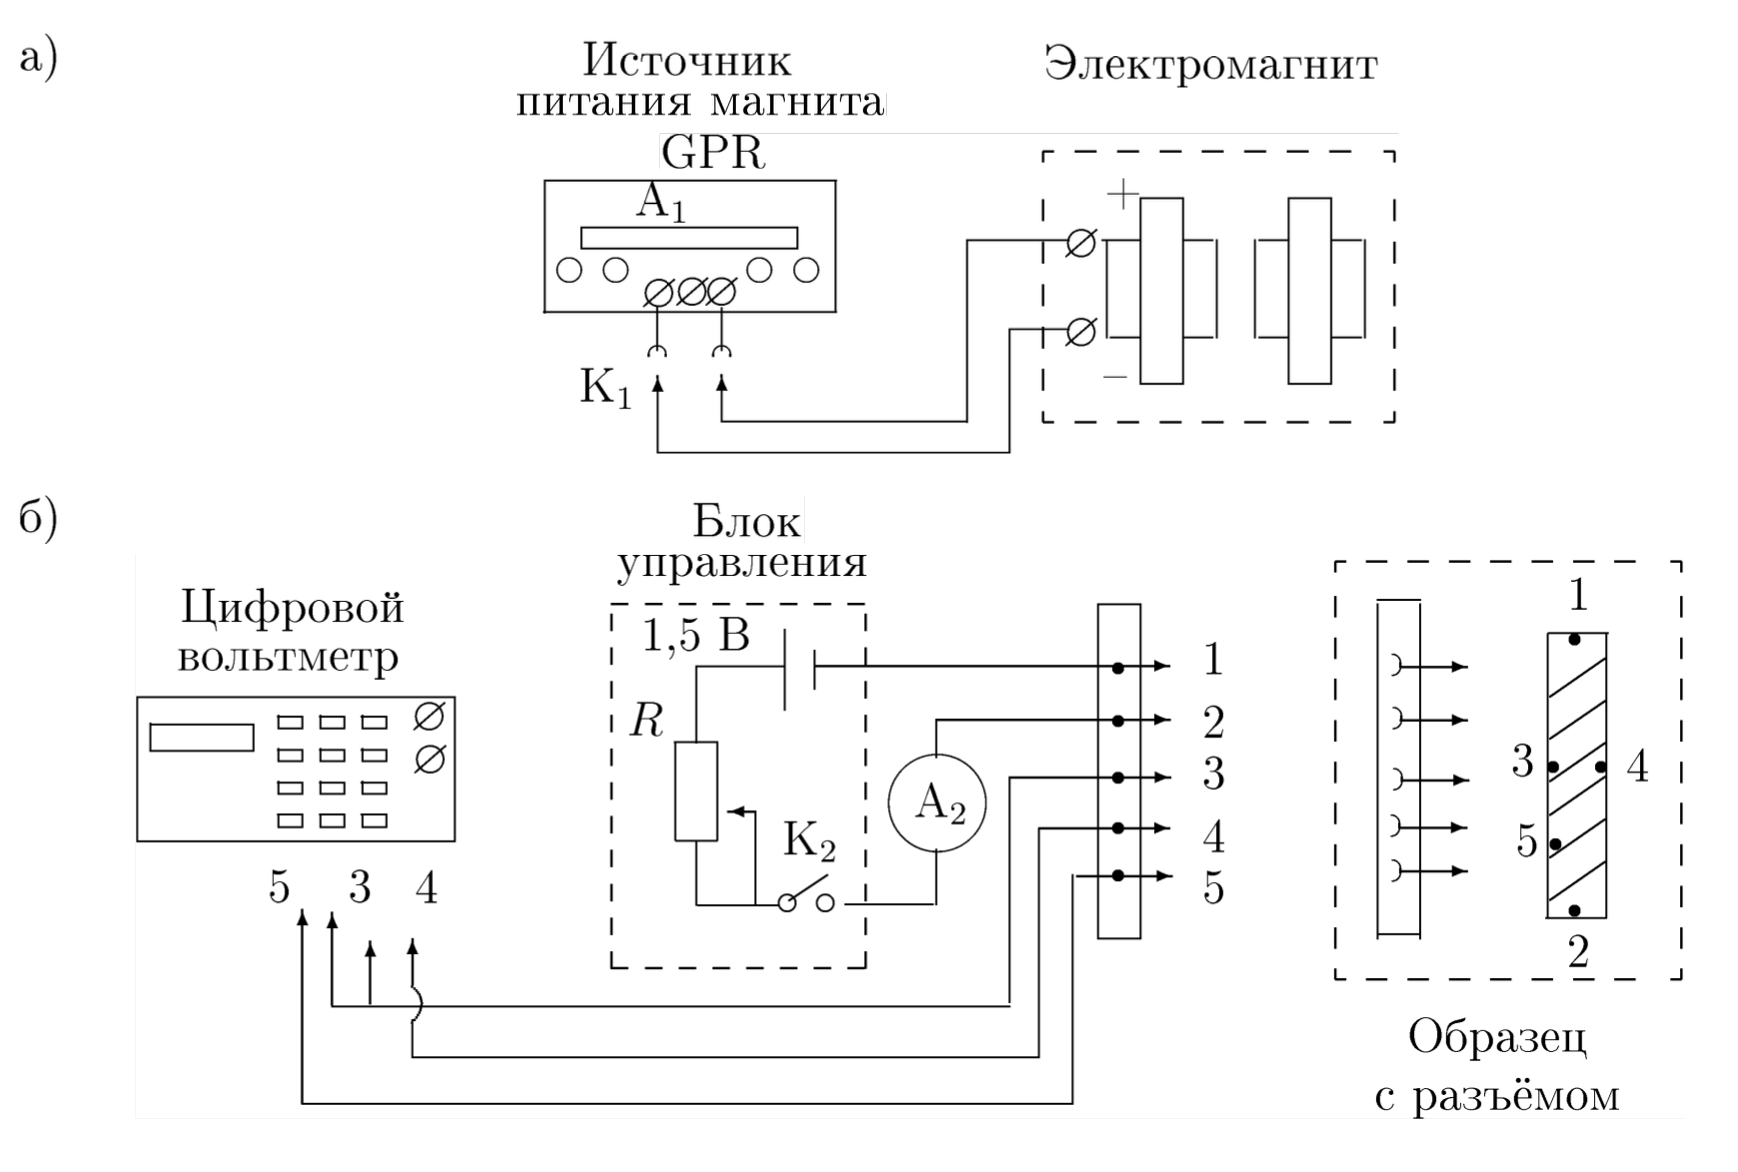
\includegraphics[width = 0.8 \textwidth]{Scheme1}
			\caption{Схема для определения динамической постоянной и критического сопротивления гальванометра}
		\end{center}
	\end {figure}

Угол отклонения рамки будем измерять с помощью осветителя, зеркальца и шкалы, находящейся на расстоянии $a$ от зеркальца. Тогда координата $x$ светового пятна будет выражаться:

$$x=a\tg(2\varphi) \approx 2a\varphi$$
Следовательно динамическая постоянная будет равна 
$$C_I = \dfrac{I}{\varphi} = \dfrac{2aI}{x}$$

Значения силы тока найдем по формуле: $$I = U_0 \dfrac{R_1}{R_2}\dfrac{1}{R+R_0}$$


\begin{table}[H]
\centering
\resizebox{\textwidth}{!}{%
\begin{tabular}{|c|c|c|c|c|c|c|c|c|c|c|c|c|c|c|c|}
\hline
$x, \text{ см}$        & 21.7  & 20.3  & 19.0   & 17.9   & 16.9   & 16.0   & 15.2   & 14.5   & 13.3   & 12.2   & 10.5   & 8.8    & 7.5    & 6.7    & 4.1    \\ \hline
$\sigma_x, \text{ см}$ & 0.5   & 0.5   & 0.5    & 0.5    & 0.5    & 0.5    & 0.5    & 0.5    & 0.5    & 0.5    & 0.5    & 0.5    & 0.5    & 0.5    & 0.5    \\ \hline
$R, \text{ Ом}$        & 800.0 & 900.0 & 1000.0 & 1100.0 & 1200.0 & 1300.0 & 1400.0 & 1500.0 & 1700.0 & 1900.0 & 2300.0 & 2900.0 & 3500.0 & 4000.0 & 7000.0 \\ \hline
$I, \text{ нА}$        & 425.5 & 397.4 & 372.7  & 350.9  & 331.5  & 314.1  & 298.5  & 284.4  & 259.7  & 239.0  & 206.2  & 170.9  & 146.0  & 130.2  & 78.8   \\ \hline
$\sigma_I, \text{ нА}$ & 7.1   & 6.6   & 6.2    & 5.8    & 5.5    & 5.2    & 5.0    & 4.7    & 4.3    & 4.0    & 3.4    & 2.8    & 2.4    & 2.2    & 1.3    \\ \hline
\end{tabular}%
}
\caption{Полученные значения}
\end{table}

	\begin {figure}[H]
		\begin{center}
%			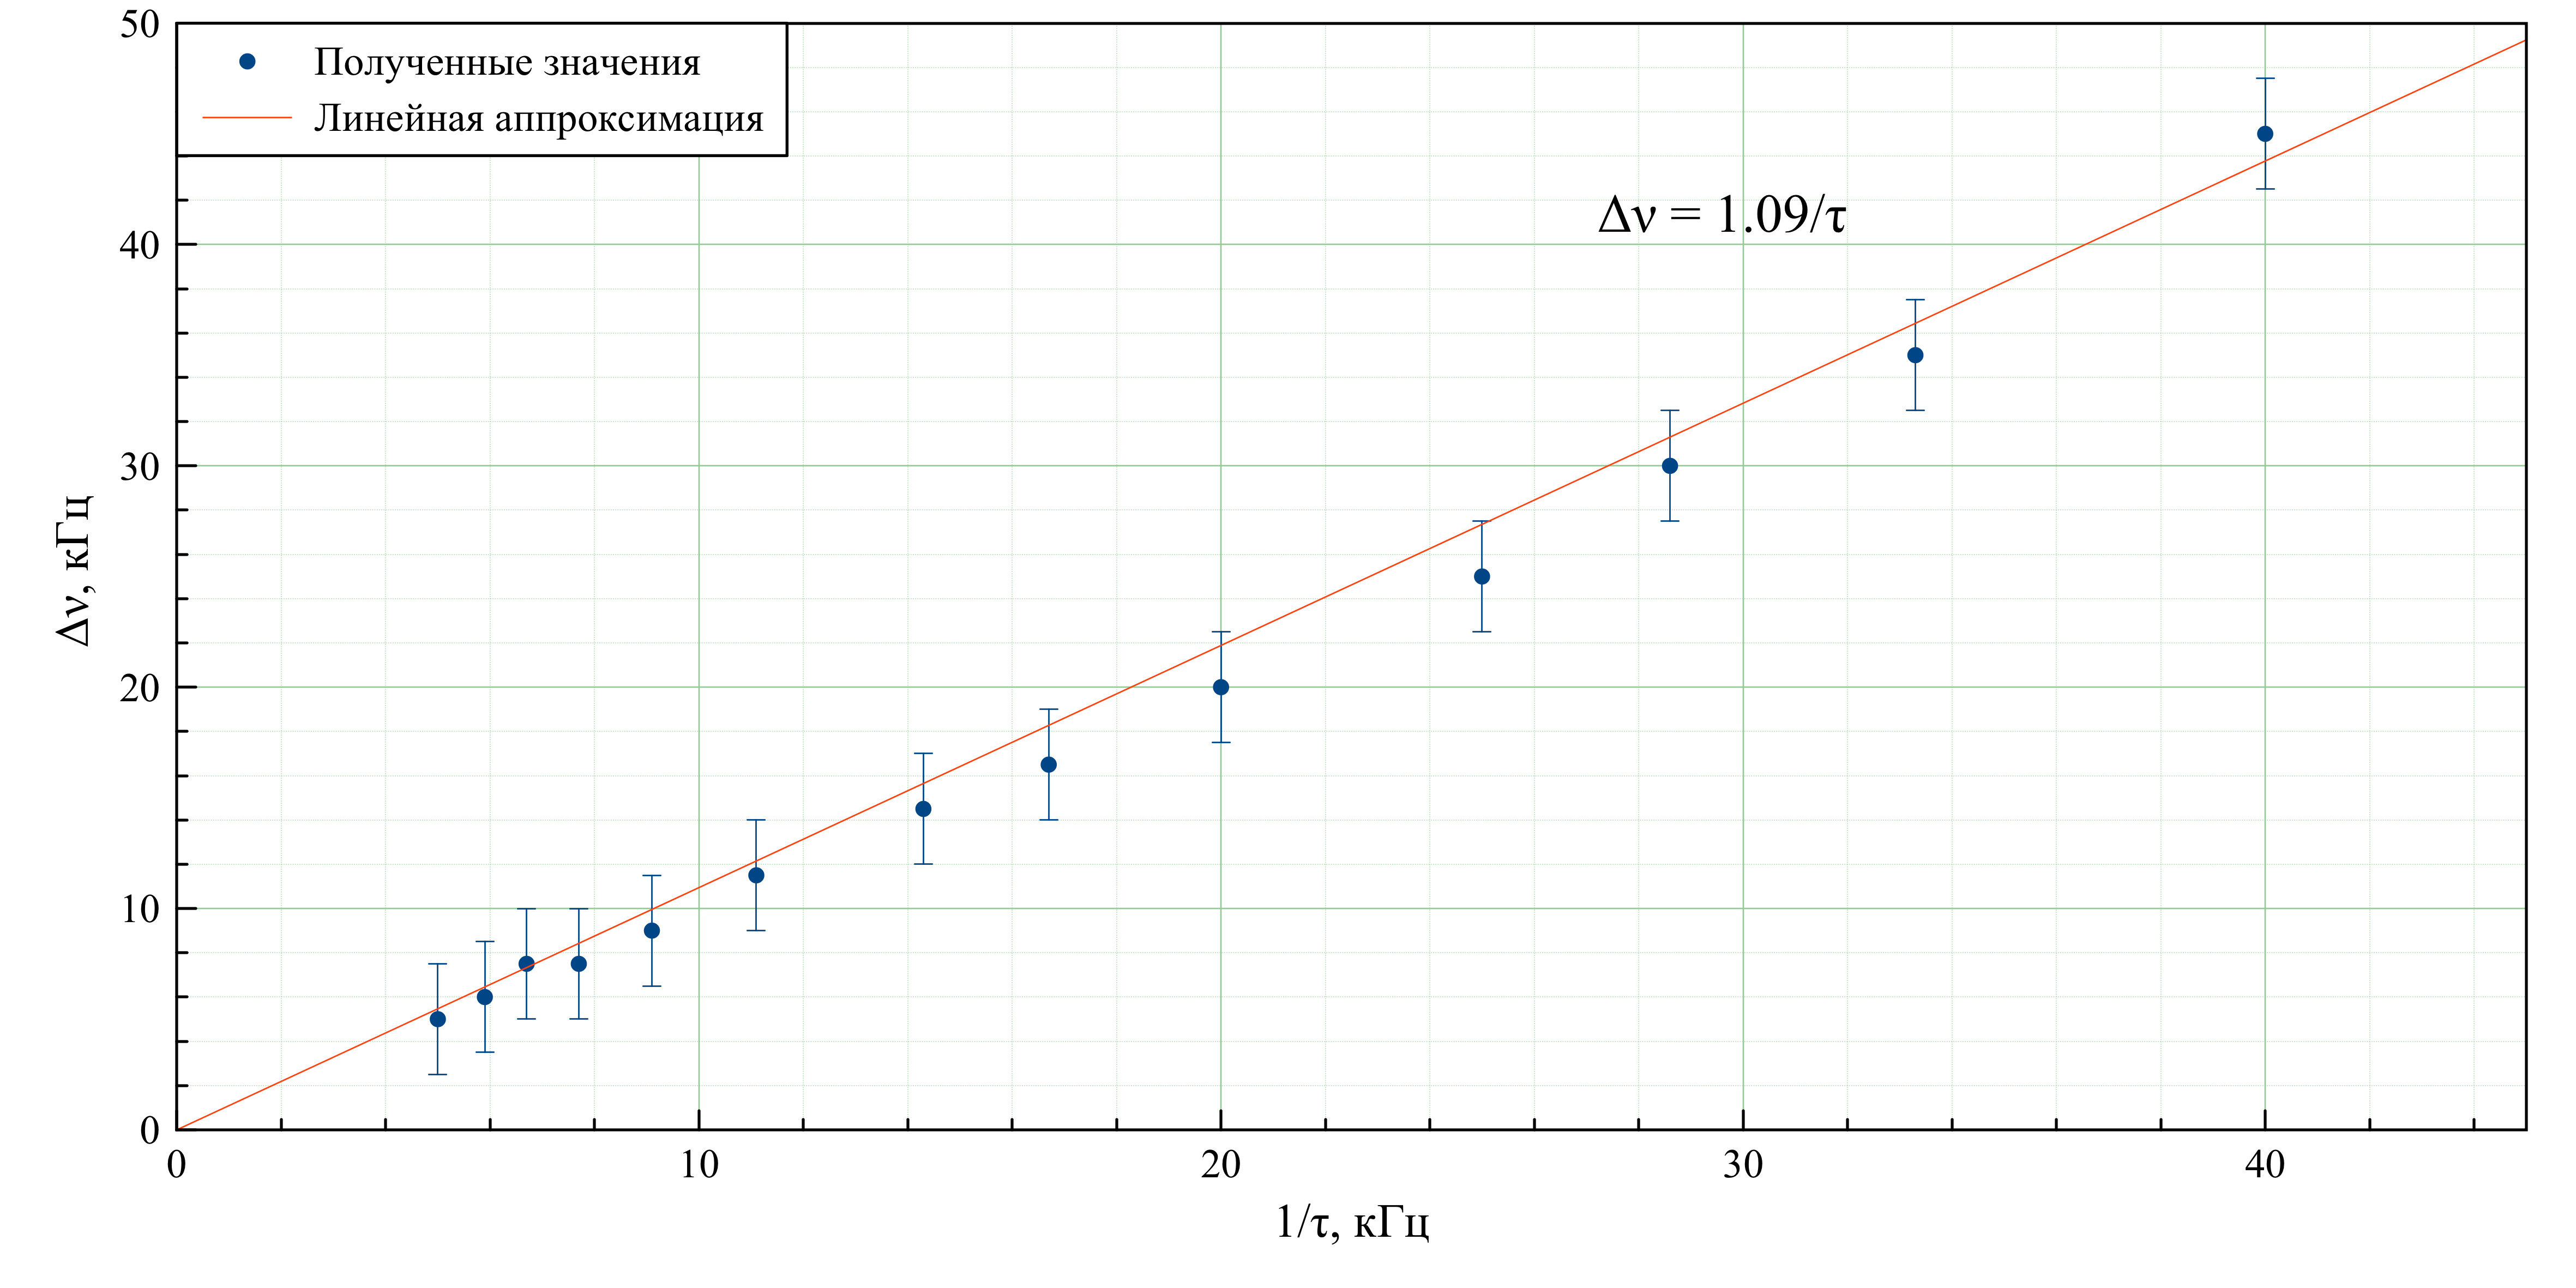
\includegraphics[width = 0.7 \textwidth]{GraphA}
			\caption{График зависимости $I = f(x)$}
		\end{center}
	\end {figure}

Получаем, что $\dfrac{C_I}{2a} = 19.7 \pm 0.7 \; \dfrac{\text{нА}}{\text{ см}}$

Тогда $C_I = 5.1 \pm 0.2 \; \dfrac{\text{нА $\cdot$ м}}{\text{ см}}$
	
\subsection*{Определение критического сопротивления}
$$R = 800.00$$
$$x_n = 18.9 \text{ см}$$
$$x_{n+1} = 16.9 \text{ см}$$
$$\Theta_0 = \ln \dfrac{x_n}{x_{n+1}} = 0.11$$	
Оценим примерное значение периода свободных колебаний:
$$T_0 = 2.38 \text{ с}$$
Оценим значение критического сопротивления, при котором зайчик не переходит за нулевое значение:
$$R_{\text{кр}} \approx 4500.0 \text{ Ом}$$

\begin{table}[H]
\centering
\begin{tabular}{|c|c|c|c|c|c|c|}
\hline
$R, \text{ кОм}$ & $x_n$ & $x_{n+1}$ & $\Theta$ & $1/\Theta^2$ & $\sigma_{1/\Theta^2}$ & $(R+R_0)^2 \text{ кОм}$ \\ \hline
15.0             & 7.8   & 0.9       & 2.16     & 0.21         & 0.02                  & 243.7                   \\ \hline
16.0             & 7.9   & 1.0       & 2.07     & 0.23         & 0.02                  & 275.9                   \\ \hline
17.0             & 7.9   & 1.1       & 1.97     & 0.26         & 0.02                  & 310.1                   \\ \hline
18.0             & 7.8   & 1.3       & 1.79     & 0.31         & 0.02                  & 346.3                   \\ \hline
19.0             & 7.6   & 1.4       & 1.69     & 0.35         & 0.02                  & 384.6                   \\ \hline
20.0             & 7.4   & 1.4       & 1.67     & 0.36         & 0.02                  & 424.8                   \\ \hline
21.0             & 7.4   & 1.5       & 1.60     & 0.39         & 0.02                  & 467.0                   \\ \hline
22.0             & 7.4   & 1.6       & 1.52     & 0.43         & 0.03                  & 511.2                   \\ \hline
25.0             & 7.0   & 1.7       & 1.42     & 0.50         & 0.03                  & 655.9                   \\ \hline
27.0             & 6.9   & 2.0       & 1.24     & 0.65         & 0.04                  & 762.3                   \\ \hline
29.0             & 6.6   & 2.0       & 1.19     & 0.70         & 0.04                  & 876.8                   \\ \hline
31.0             & 6.4   & 2.2       & 1.07     & 0.88         & 0.06                  & 999.2                   \\ \hline
34.0             & 6.1   & 2.2       & 1.02     & 0.96         & 0.06                  & 1197.9                  \\ \hline
37.0             & 5.7   & 2.2       & 0.95     & 1.10         & 0.08                  & 1414.5                  \\ \hline
40.0             & 5.5   & 2.3       & 0.87     & 1.32         & 0.10                  & 1649.2                  \\ \hline
43.0             & 5.3   & 2.3       & 0.83     & 1.43         & 0.12                  & 1901.8                  \\ \hline
46.0             & 4.9   & 2.3       & 0.76     & 1.75         & 0.16                  & 2172.5                  \\ \hline
49.0             & 4.7   & 2.3       & 0.71     & 1.96         & 0.19                  & 2461.2                  \\ \hline
\end{tabular}
\caption{Исследование зависимости $\Theta$ от $R$}
\end{table}

\begin{equation}
\Theta = \gamma T = 2 \pi \dfrac{\gamma}{\omega} = \dfrac{2 \pi \gamma}{\sqrt{\omega_0^2 - \gamma^2}} = \dfrac{2 \pi R_3}{\sqrt{R_\Sigma^2 - R_3^2}},
\label{eq:critical}
\end{equation}
где введено обозначение:
$$R_3 = \frac{(BSN)^2}{2\sqrt{JD}} = R_0 + R_\text{кр}$$
Тогда при $R = R_\text{кр}$  выполняется: $\Theta \rightarrow \infty$

Получим из \ref{eq:critical} уравнение прямой в координатах $X = (R_0 + R)^2$ и $Y = 1/\Theta^2$:

$$\dfrac{1}{\Theta^2} = \dfrac{(R_0 + R)^2}{4 \pi^2 R_2^3} - \dfrac{1}{4 \pi^2}$$

Тогда $R_\text{кр} = \dfrac{1}{2 \pi} \sqrt{\dfrac{\Delta X}{\Delta Y}} - R_0$

\begin {figure}[H]
	\begin{center}
%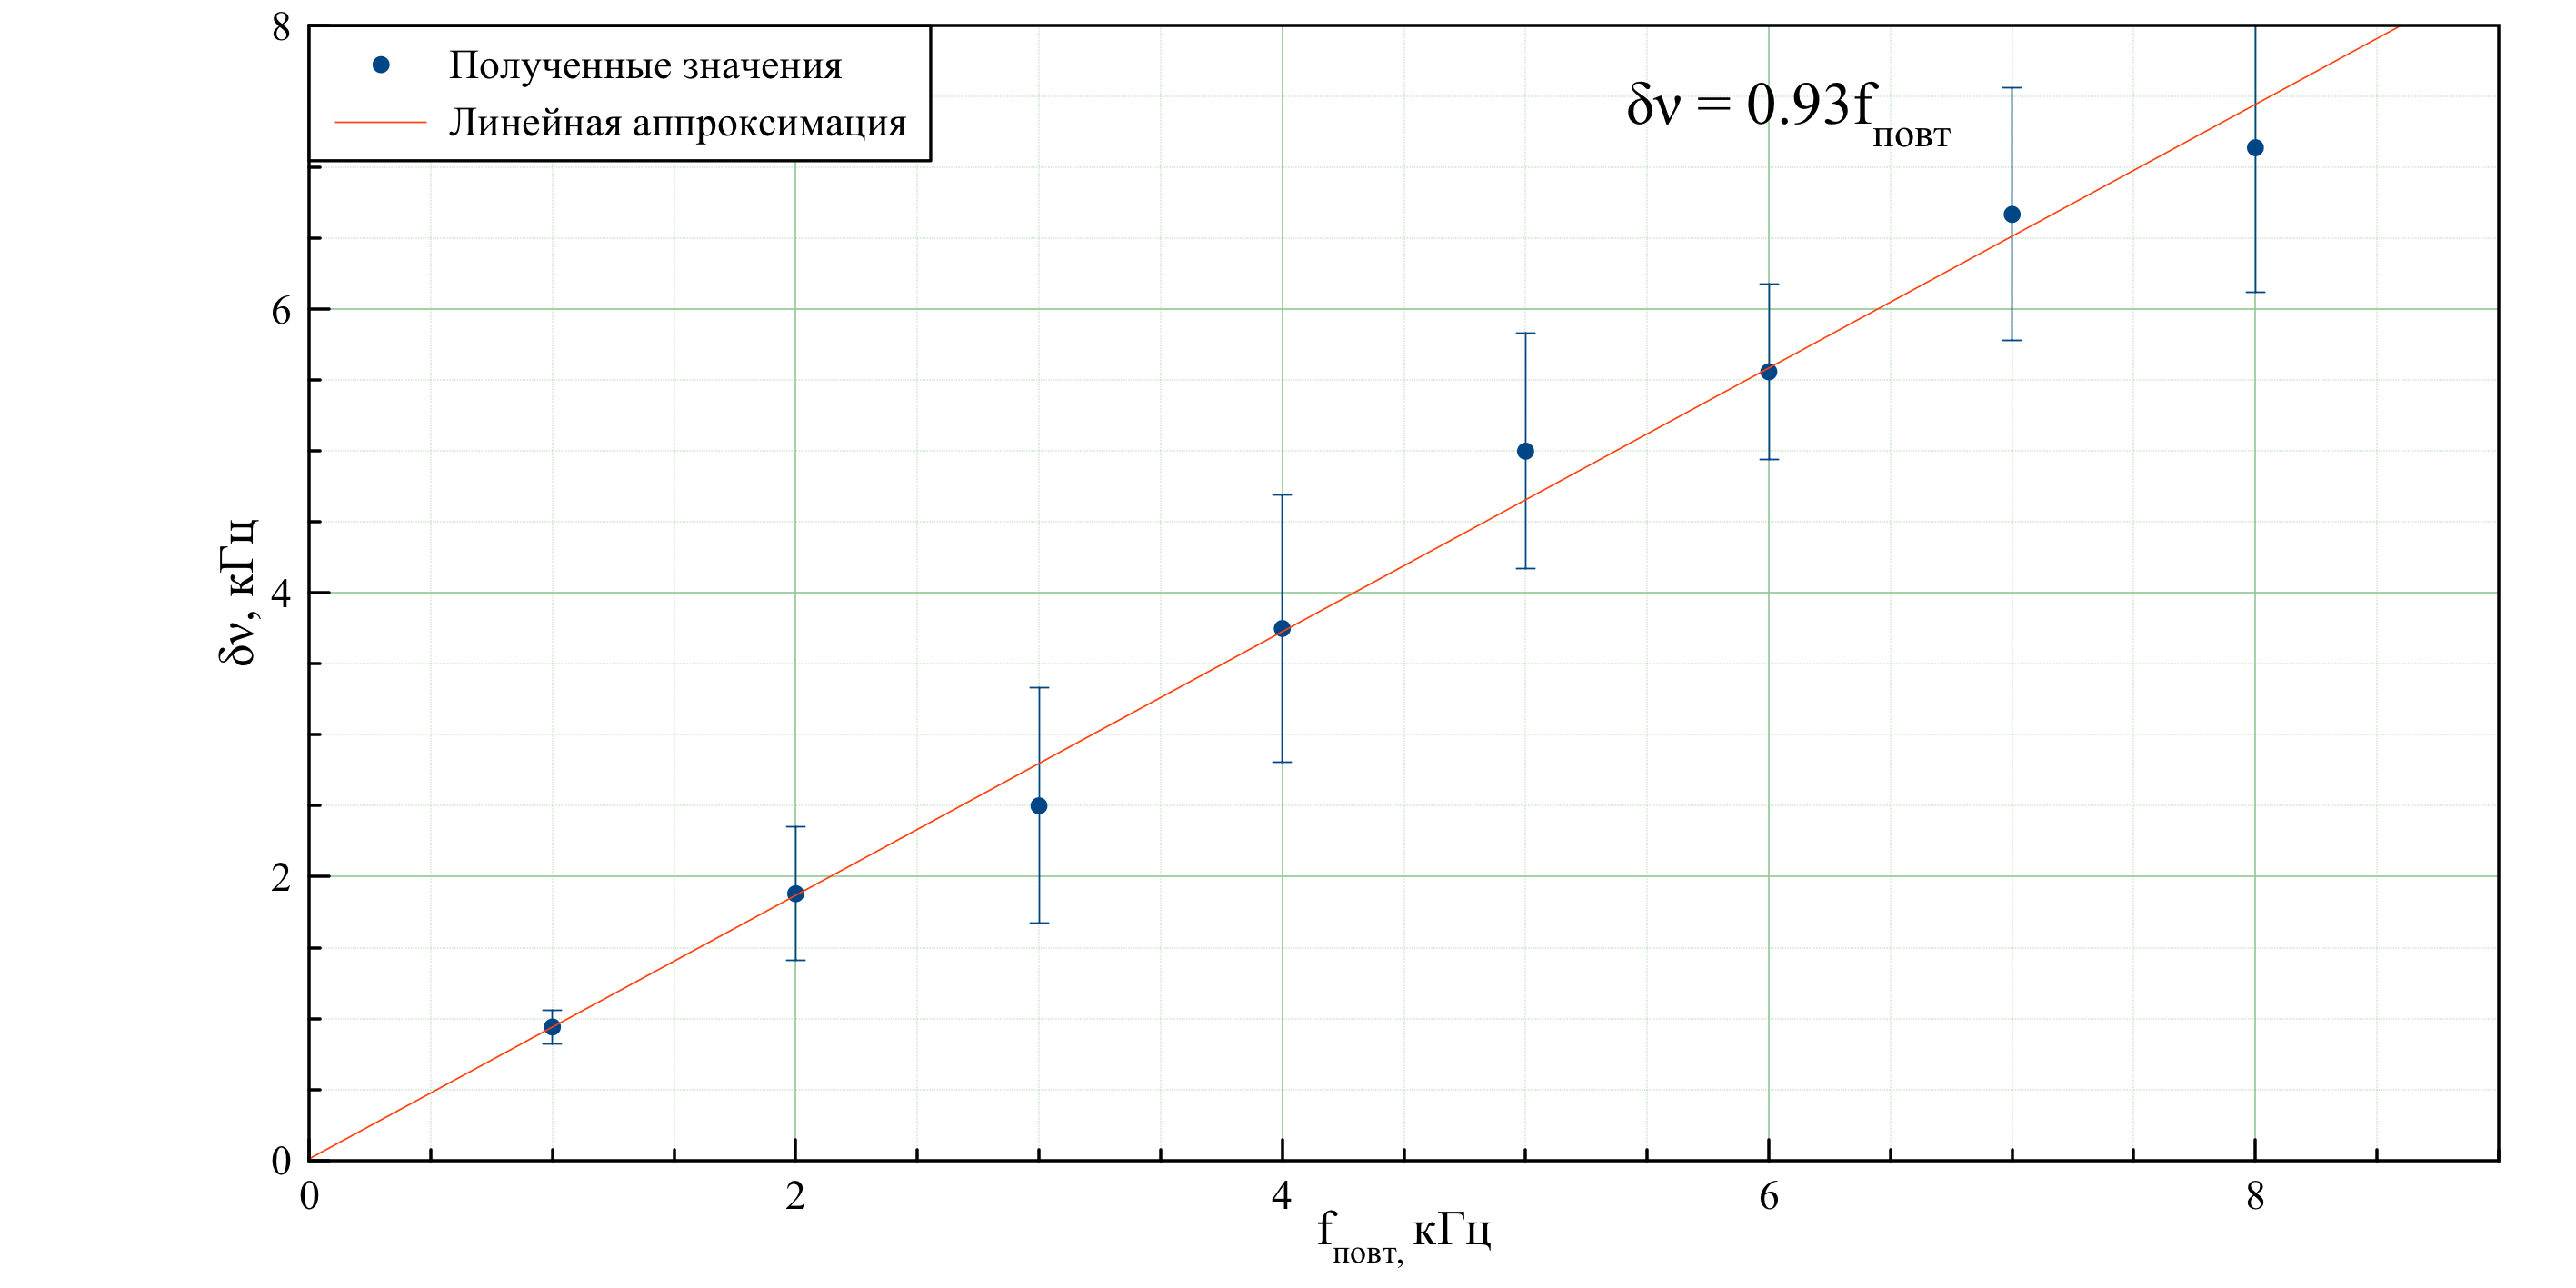
\includegraphics[width = 0.7\textwidth]{GraphB}
		\caption{График зависимости $1/\Theta^2 = f((R_0 + R)^2)$ в области малых R}
	\end{center}
\end {figure}


Из графика $\dfrac{\Delta X}{\Delta Y} = 1.1 \pm 0.1 \text{ (10 кОм)}^2$, поэтому 
$$R_\text{кр} = 4785 \pm 290 \text{ Ом}$$

\subsection*{Баллистический режим}

$$C = 2 \text{ мкФ}$$
$$R_1/R_2 = 1/2$$
$$l_max = 18.7 \text{ см}$$

Соберем схему:

\begin {figure}[H]
	\begin{center}
%		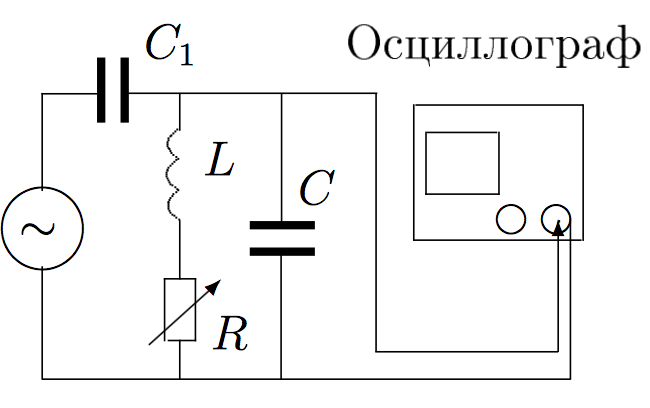
\includegraphics[width = 0.8 \textwidth]{Scheme2}
		\caption{Схема для определения баллистической постоянной и критического сопротивления гальванометра, работающего в баллистическом режиме}
	\end{center}
\end {figure}

\begin{table}[H]
\centering
\begin{tabular}{|c|c|c|c|}
\hline
$R, \text{ Ом}$ & $l_{max}$ & $\sigma_{l_{max}}$ & $(R+R_0)^{-1}, \; 10^6 \; \text{Ом}^{-1}$ \\ \hline
30000.0         & 13.6      & 0.4                & 3.3            \\ \hline
25000.0         & 13.2      & 0.4                & 3.9            \\ \hline
20000.0         & 12.8      & 0.4                & 4.9            \\ \hline
15000.0         & 11.6      & 0.4                & 6.4            \\ \hline
10000.0         & 9.5       & 0.4                & 9.4            \\ \hline
9000.0          & 9.3       & 0.4                & 10.4           \\ \hline
8000.0          & 8.8       & 0.4                & 11.6           \\ \hline
7000.0          & 8.2       & 0.4                & 13.1           \\ \hline
6000.0          & 7.7       & 0.4                & 15.1           \\ \hline
5000.0          & 6.9       & 0.4                & 17.8           \\ \hline
\end{tabular}
\caption{Исследуем зависимость между $l_{max}$ и $R$}
\end{table}

\begin {figure}[H]
	\begin{center}
%		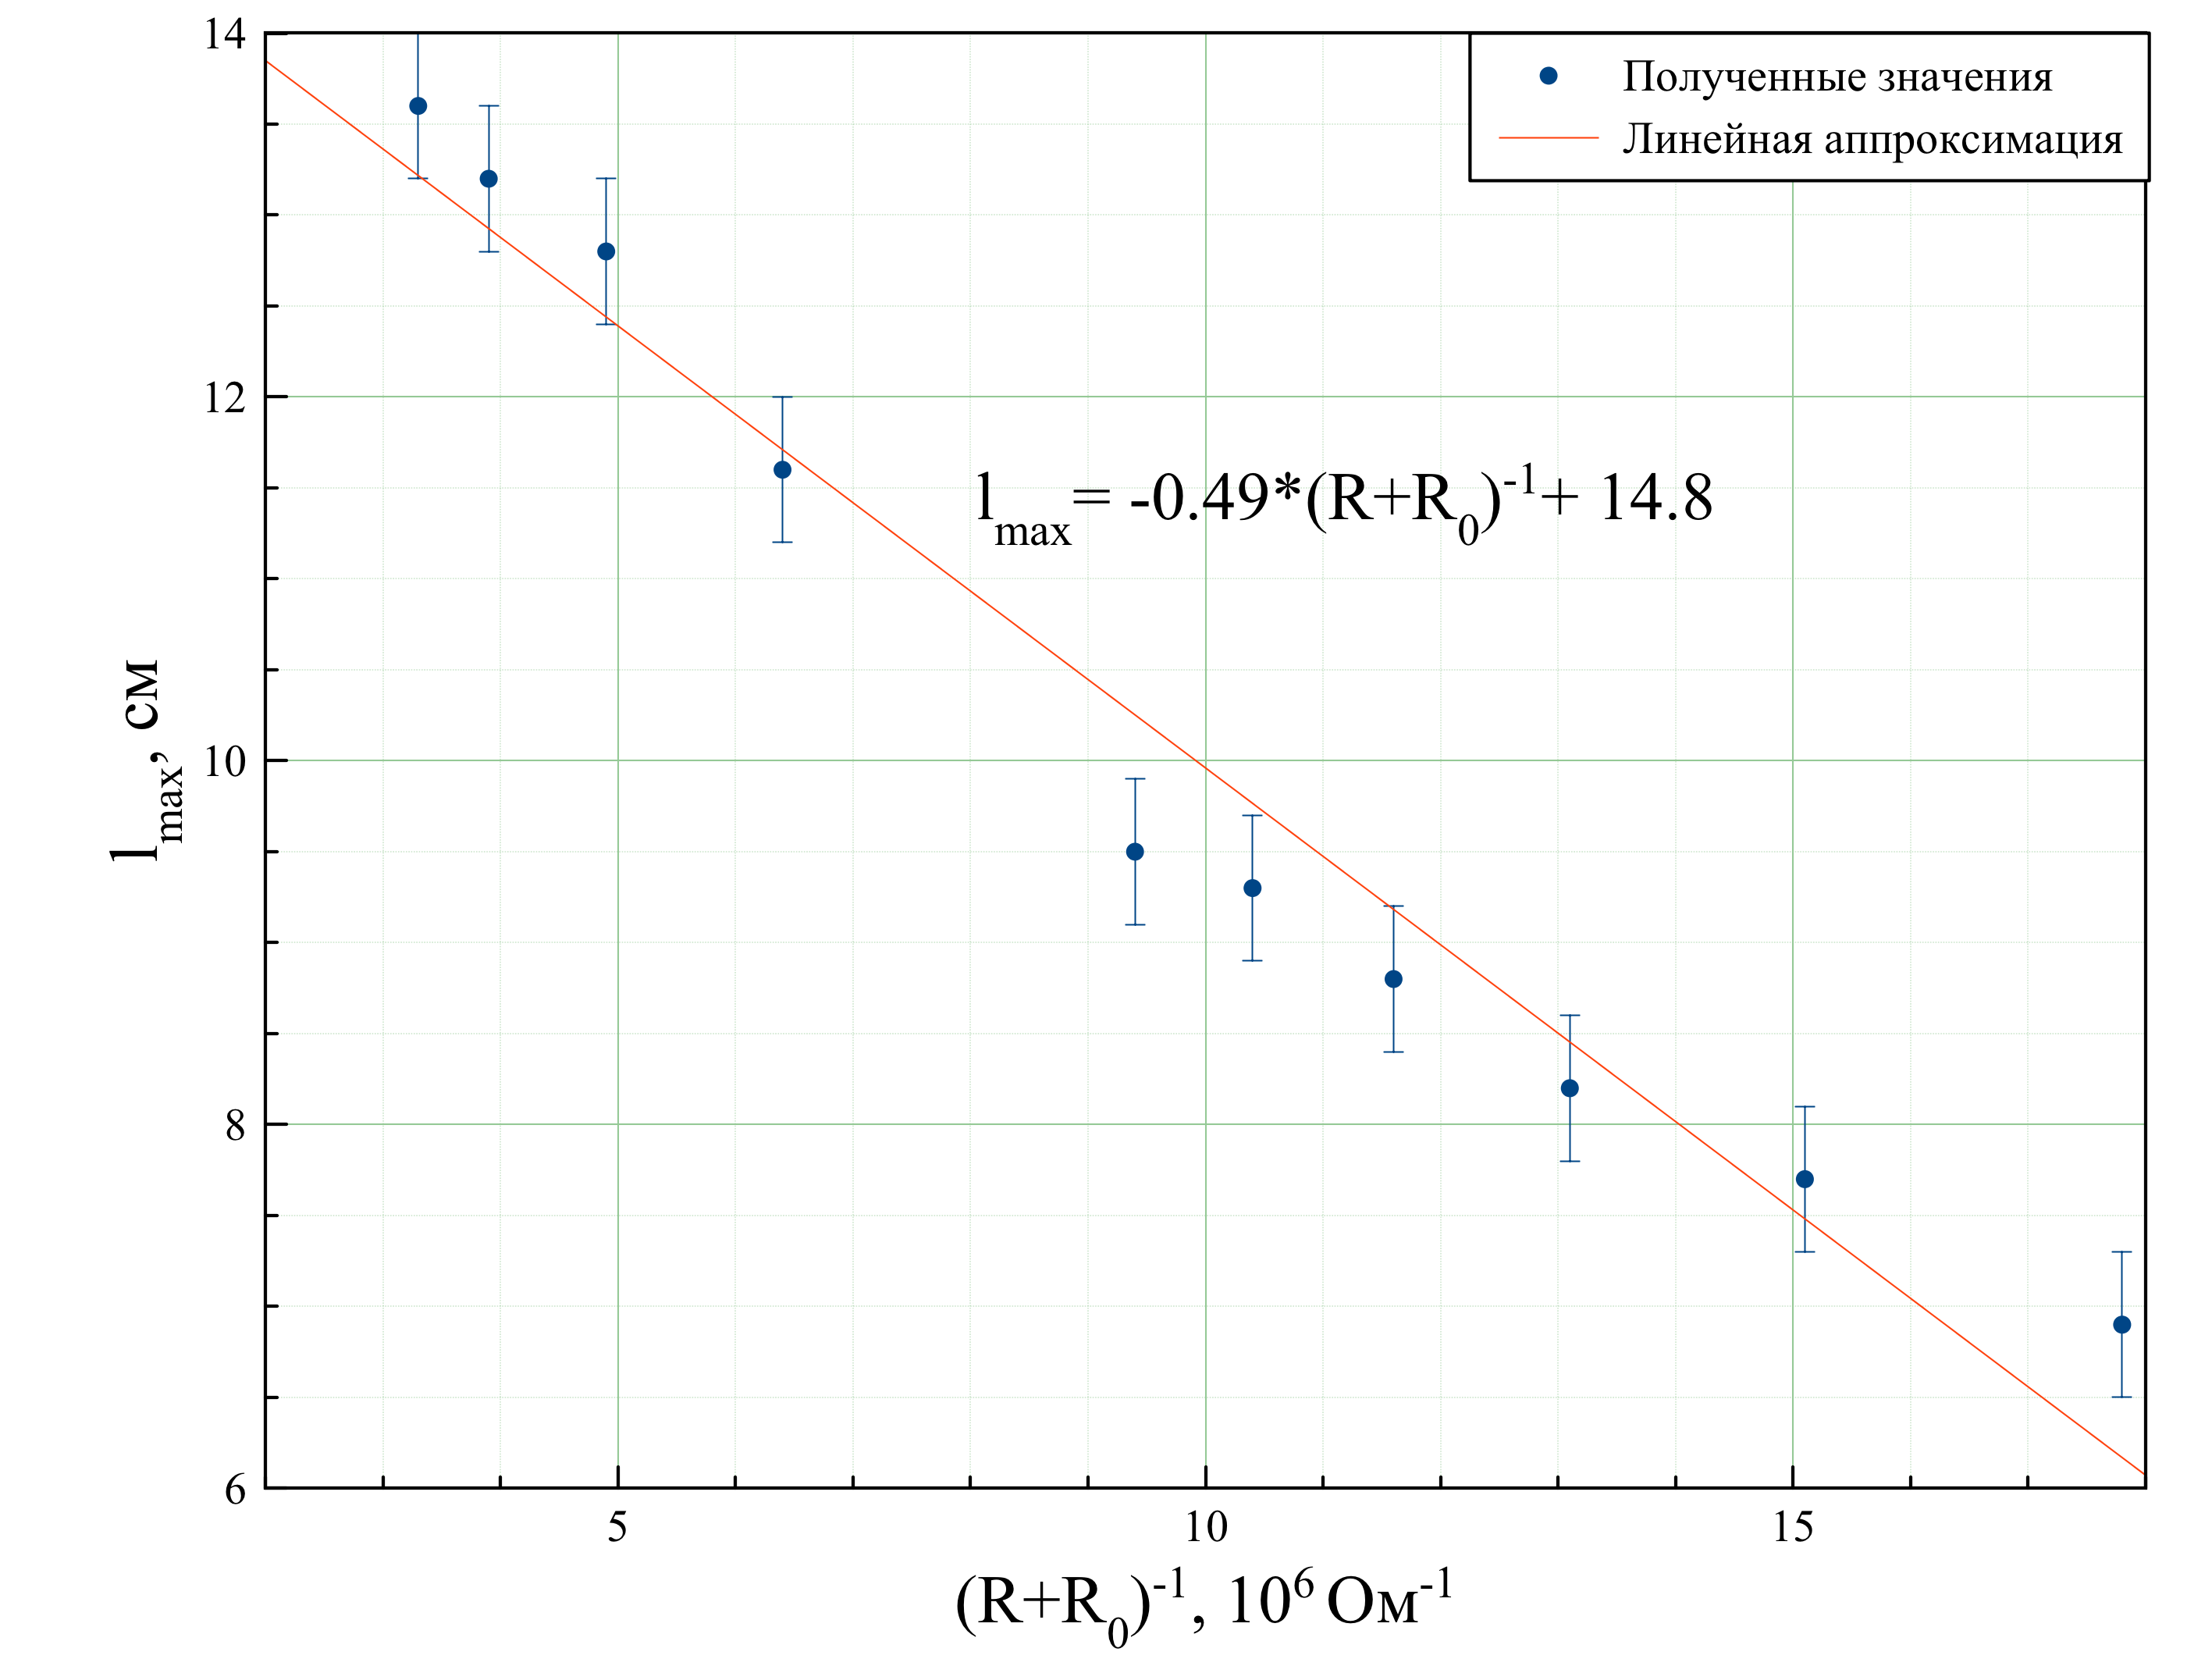
\includegraphics[width = 0.8 \textwidth]{GraphC}
		\caption{Зависимость $l_{max} = f[(R_0+R)^{-1}]$}
	\end{center}
\end {figure}

Определим значение $R_\text{кр}$ по графику: значение максимального отклонения в критическом режиме в $e$ раз меньше, чем в режиме свободных колебаний. Зная зависимость $l_{max} = f[(R_0+R)^{-1}]$ найдем значение сопротивления, соответствующее 
$$R_\text{кр} = R(l_{max}/e) = 4950 \pm 340 \text{ Ом}$$

Определим баллистическую постоянную гальванометра $C_{Q_\text{кр}} \left[\dfrac{\text{К}}{\text{мм/м}} \right]$:

$$C_{Q_\text{кр}} = \dfrac{q}{\varphi_{max \text{ кр}}} = 2a \dfrac{R_1}{R_2} \dfrac{U_0C}{l_{max \text{ кр}}} = 17 \pm 0.7 \; \text{м$\cdot$нК/мм}$$

Время релаксации $t = R_0C = 610 \cdot 2 \cdot 10^{-6} = 1.22 \cdot 10^{-3} \text{ с} \ll T_0 = 2.8 \text{ с}$

\section{Вывод}

В данной лабораторной работе мы измерили значение динамической постоянной гальванометра, критического сопротивления тремя способами и баллистической постоянной. В измерениях динамической постоянной значения $R_\text{кр}$ совпадают с учетом погрешности. Наибольшая погрешность в третьем эксперименте, так как большой вклад в погрешность дает скорость реакции человека (отклонения зайчика происходят быстро, необходимо успевать замыкать ключ и считывать значения).

\end{document}